\section{Methods}

This retrospective study included 12,400 colour fundus photographs collected at two tertiary hospitals between 2019 and 2023.
The study was approved by the institutional review board (IRB-0000-00), and the requirement for informed consent was waived because all images were de-identified.
Each image was independently labelled by two certified graders; disagreements were resolved by a senior ophthalmologist.

Fig.~\ref{fig:overview} illustrates the overall pipeline of LesionTriage, which consists of two stages.
The first stage detects haemorrhages, microaneurysms and exudates; the second stage grades referral urgency from the detected lesions.
The network was optimised with a weighted cross-entropy loss, defined as Eq.~(\ref{eq:loss}).

\begin{equation}
\mathcal{L} = -\sum_{c=1}^{C} w_c \, y_c \log \hat{y}_c
\label{eq:loss}
\end{equation}

\begin{figure}[t]
\centering
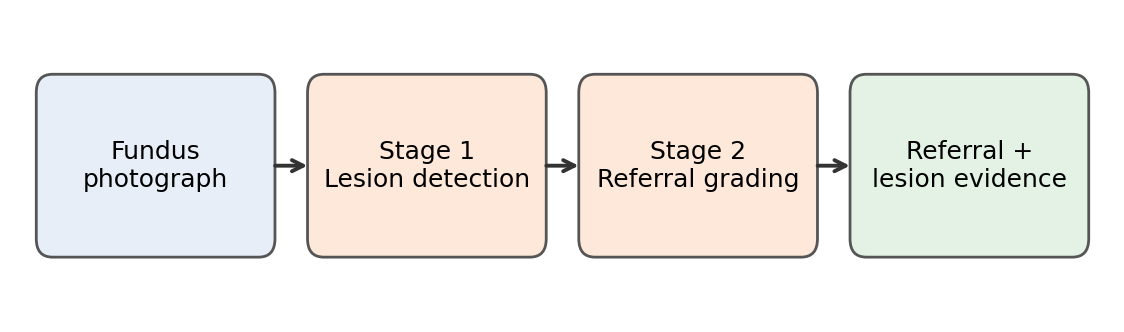
\includegraphics[width=\linewidth]{figures/overview.png}
\caption{Overview of LesionTriage: lesion detection followed by referral grading.}
\label{fig:overview}
\end{figure}

The model was trained for 60 epochs with AdamW, a learning rate of $3 \times 10^{-4}$ and a batch size of 16.
Performance was measured by AUC, sensitivity and specificity, with 95\% confidence intervals from 2,000 bootstrap samples \citep{efron2020bootstrap}.
